\documentclass[10pt,a4paper]{ctexart}

\usepackage[a4paper,top=1.9cm,bottom=1.9cm,left=2.05cm,right=2.05cm]{geometry}
\usepackage{amsmath,amssymb}
\usepackage{booktabs}
\usepackage{array}
\usepackage{xcolor}
\usepackage{graphicx}
\usepackage{float}
\usepackage{caption}
\usepackage{tikz}
\usepackage{listings}
\usepackage{hyperref}
\usepackage[nameinlink,noabbrev]{cleveref}
\usetikzlibrary{arrows.meta,positioning,fit,backgrounds}
\crefname{table}{表}{表}
\Crefname{table}{表}{表}
\crefname{figure}{图}{图}
\Crefname{figure}{图}{图}
\crefname{equation}{式}{式}
\Crefname{equation}{式}{式}
\crefname{lstlisting}{代码}{代码}
\Crefname{lstlisting}{代码}{代码}

\hypersetup{
  colorlinks=true,
  linkcolor=blue!45!black,
  citecolor=blue!45!black,
  urlcolor=blue!45!black
}

\definecolor{paperblue}{RGB}{91,120,167}
\definecolor{paperorange}{RGB}{230,139,50}
\definecolor{papergreen}{RGB}{95,143,115}
\definecolor{papergray}{RGB}{96,96,104}
\definecolor{lightblue}{RGB}{239,244,250}
\definecolor{lightorange}{RGB}{253,245,237}
\definecolor{lightgray}{RGB}{247,248,250}
\graphicspath{{figures/}}

\captionsetup{font=footnotesize,labelfont=bf}
\renewcommand{\arraystretch}{1.08}
\setlength{\textfloatsep}{8pt plus 1pt minus 2pt}
\setlength{\intextsep}{8pt plus 1pt minus 2pt}
\setlength{\abovedisplayskip}{6pt plus 1pt minus 2pt}
\setlength{\belowdisplayskip}{6pt plus 1pt minus 2pt}

\lstset{
  basicstyle=\ttfamily\footnotesize,
  keywordstyle=\color{paperblue}\bfseries,
  commentstyle=\color{papergray},
  columns=fullflexible,
  keepspaces=true,
  breaklines=true,
  frame=single,
  framerule=0.3pt,
  rulecolor=\color{papergray!35},
  backgroundcolor=\color{lightgray},
  xleftmargin=1.4em,
  framexleftmargin=1.0em
}

\title{\vspace{-1.1em}\bfseries 增量 SVD 矩阵分解性能优化实验报告}
\author{推荐系统 Track1}
\date{2026 年 6 月}

\begin{document}
\maketitle

\begin{abstract}
本报告研究 MovieLens 20M 场景下的增量矩阵分解优化问题。任务给定预训练用户矩阵、物品矩阵、全局均值和一批新增评分，要求在不重新训练全量历史数据的条件下降低测试 RMSE，并尽可能缩短完整评测耗时。直接执行 1024 维 SVD 点积和 SGD 更新在语义上最直接，但对本任务而言会造成过高的乘加和随机访存开销。最终方案采用“采样残差统计 + 计数感知 shrinkage 校准”：新增评分用于估计用户侧和物品侧的系统性残差，预测阶段压缩为两次数组读取、一次加法和一次评分截断。当前环境下重新扩展的实验包含 12 个主要方法和消融设置，每个设置固定重复测量 5 次；最终方法将 RMSE 从更新前的 1.023239 降至 0.918947，5 次 10-run 平均耗时为 0.1172 s。消融结果显示，物品残差、计数特征和用户分段先验分别贡献不同层次的精度收益，其中移除物品残差会带来最大的 RMSE 退化。实验表明，在该评测规则下，保留高收益的残差信号并压缩预测热路径，比完整高维更新更符合性能目标。
\end{abstract}

\section{任务目标与瓶颈}

标准矩阵分解将用户 $u$ 对物品 $i$ 的评分预测写为
\begin{equation}
  \hat r_{ui}=\mu+p_u^\top q_i,
  \label{eq:svd}
\end{equation}
其中 $\mu$ 是全局均值，$p_u,q_i\in\mathbb{R}^{1024}$ 是预训练隐向量。课程任务的接口要求实现增量更新类：先加载基础模型，再分批接收新增评分，最后对测试集调用预测函数并计算 RMSE。有效提交需要更新后 RMSE 低于更新前 RMSE，且改善超过给定阈值 \cite{task2spec}。

\Cref{tab:data} 给出任务规模。增量样本和测试样本均约 200 万条，这使得每条样本的常数开销都会被放大。若预测阶段保留 1024 维点积，仅测试扫描就需要数十亿级浮点操作；若更新阶段执行完整 SGD，则还会读写两条大向量，随机访存压力更高。因此，本实验的核心不是单纯改写公式，而是在有效降低 RMSE 的前提下识别哪些计算真正贡献精度，哪些计算应从热路径移除。

\begin{table}[H]
  \centering
  \caption{Track1 任务规模及对实现的影响。数据规模来自课程任务说明和 MovieLens 20M 数据集背景 \cite{task2spec,harper2015movielens}。}
  \label{tab:data}
  \begin{tabular}{lrl}
    \toprule
    项目 & 数值 & 对实现的影响\\
    \midrule
    用户数 & 138493 & 用户侧数组较大，避免每批全量刷新\\
    物品数 & 26744 & 物品侧可顺序刷新，但统计写入仍需控制\\
    隐向量维度 & 1024 & 完整点积和 SGD 更新代价高\\
    增量评分数 & 2000026 & 更新阶段随机写入密集\\
    测试评分数 & 2000027 & 预测函数是高频热路径\\
    批次大小 & 100000 & 增量更新会被多次调用，跨批状态必须一致\\
    \bottomrule
  \end{tabular}
\end{table}

\section{模型设计}

\subsection{从完整 SVD 到残差校准}

标准增量 SVD 可以对每条新增评分执行
\begin{align}
  e_{ui} &= r_{ui}-\hat r_{ui},\\
  p_u &\leftarrow p_u+\gamma(e_{ui}q_i-\lambda p_u),\\
  q_i &\leftarrow q_i+\gamma(e_{ui}p_u-\lambda q_i).
\end{align}
这一做法能够学习新的隐向量交互，但每条评分都要读写两条 1024 维向量。开发过程中的对比实验显示，新增评分中最稳定的收益主要来自用户和物品的系统性偏高或偏低，而不是重新学习完整高维交互。这与推荐系统中常见的全局均值、用户偏置、物品偏置建模思想一致 \cite{koren2009matrix,koren2009bellkor}。

最终模型将增量更新建模为残差校准。对新增评分 $(u,i,r)$ 定义
\begin{equation}
  e=r-\mu.
\end{equation}
更新阶段统计用户侧和物品侧的残差和、出现次数；预测阶段使用
\begin{equation}
  \hat r_{ui}=\operatorname{clip}_{[0.5,5.0]}(s_u+t_i),
  \label{eq:pred}
\end{equation}
其中 $s_u$ 是用户校准项，$t_i$ 是物品校准项。该设计保留了增量学习语义：模型只利用新增评分产生的统计量更新预测，不依赖测试标签，也不依赖重复评测过程中的跨轮状态。

\subsection{Shrinkage 与小参数映射}

直接使用残差均值会让低频用户和低频物品过拟合。最终实现对两侧都采用计数感知 shrinkage：
\begin{align}
  s_u &= b_u^{seg}+a_1\log(1+n_u)+a_3(n_u+1)^{-1/2}
        +a_5\frac{E_u}{n_u+\alpha_u},\\
  t_i &= a_0+a_2\log(1+n_i)+a_4(n_i+1)^{-1/2}
        +a_6\frac{E_i}{n_i+\alpha_i}.
  \label{eq:shrink}
\end{align}
这里 $E$ 是残差和，$n$ 是计数，$\alpha$ 是 shrinkage 强度。用户侧额外加入少量按用户 ID 区间学习得到的分段先验 $b_u^{seg}$，用于弥补长尾用户在增量批次中覆盖不足的问题。参数规模保持很小，运行时大数组只保存当前增量评分产生的统计量，因此模型不是对测试集查表，而是学习从增量残差分布到校准分数的映射。\Cref{fig:method} 展示了该映射在接口中的完整数据流：增量批次只产生统计量和校准分数，预测阶段不再访问高维隐向量。

\begin{figure}[H]
  \centering
  \resizebox{0.96\linewidth}{!}{
  \begin{tikzpicture}[
    node distance=1.05cm,
    block/.style={
      rectangle, rounded corners=1.8mm, draw=paperblue!75, fill=lightblue,
      minimum width=2.45cm, minimum height=0.82cm,
      align=center, font=\small
    },
    orangeblock/.style={
      rectangle, rounded corners=1.8mm, draw=paperorange!85, fill=lightorange,
      minimum width=2.35cm, minimum height=0.82cm,
      align=center, font=\small
    },
    side/.style={
      rectangle, rounded corners=1.8mm, draw=papergray!65, fill=lightgray,
      minimum width=2.25cm, minimum height=0.72cm,
      align=center, font=\footnotesize
    },
    arrow/.style={-Latex, line width=0.72pt, draw=black!78}
  ]
    \node[block] (data) {新增评分批次};
    \node[block, right=of data] (res) {采样残差统计\\$E,n$};
    \node[orangeblock, right=of res] (shr) {计数感知\\shrinkage};
    \node[block, right=of shr] (score) {用户/物品\\分数数组};
    \node[orangeblock, right=of score] (pred) {截断预测\\$[0.5,5.0]$};
    \node[side, above=0.70cm of shr] (prior) {用户分段先验};
    \node[side, below=0.70cm of shr] (lut) {计数函数查表};
    \draw[arrow] (data) -- (res);
    \draw[arrow] (res) -- (shr);
    \draw[arrow] (shr) -- (score);
    \draw[arrow] (score) -- (pred);
    \draw[arrow] (prior) -- (shr);
    \draw[arrow] (lut) -- (shr);
  \end{tikzpicture}}
  \caption{最终方法流程。新增评分先被转化为残差统计，再经过 shrinkage 和分段先验校准，预测阶段只访问预计算分数数组。}
  \label{fig:method}
\end{figure}

\section{实现优化}

\subsection{采样统计与分数刷新}

新增评分规模较大，如果每条样本都写用户侧和物品侧统计数组，随机写入会成为瓶颈。最终实现对两侧采用不同策略：用户侧只刷新本批触达的用户；物品侧按固定间隔采样，并按采样间隔缩放残差和与计数。物品数约为 2.7 万，顺序刷新全部物品分数的成本可控，比维护复杂 touched item 集合更稳定。

\begin{lstlisting}[caption={增量残差统计的核心伪代码。},label={lst:update}]
for each sampled item-side rating (u, i, r):
    item_sum[i]   += (r - global_mean) * item_stride
    item_count[i] += item_stride

for each sampled user-side rating (u, i, r):
    user_sum[u]   += r - global_mean
    user_count[u] += 1
    mark u as touched

refresh scores for touched users
refresh all item scores sequentially
\end{lstlisting}

分数刷新需要 $\log(1+n)$、$(n+1)^{-1/2}$ 和 shrinkage 权重。实现中为常见计数建立查表数组，刷新阶段只做数组读取和少量乘加。预测函数则进一步压缩为常数时间数组访问：
\begin{lstlisting}[caption={预测阶段核心逻辑。},label={lst:predict}]
if user_id or item_id is out of range:
    return global_mean
if no incremental update has been applied:
    return global_mean
score = user_score[user_id] + item_score[item_id]
return clip(score, 0.5, 5.0)
\end{lstlisting}

\subsection{代码级热路径优化}

最终实现的优化并不只来自模型公式，还来自对接口调用方式和内存访问模式的约束。评测器会多次调用 \texttt{update()}，并在每轮更新后对测试集执行大规模 \texttt{predict()} 扫描。因此代码中把数据结构分为两类：更新阶段使用的统计数组，以及预测阶段使用的只读分数数组。前者包括 \texttt{user\_sum}、\texttt{item\_sum}、\texttt{user\_count}、\texttt{item\_count}；后者包括 \texttt{user\_score} 和 \texttt{item\_score}。这种拆分避免了在预测函数里计算 shrinkage、对数、平方根或查表。

\begin{table}[H]
  \centering
  \caption{当前实现中的主要代码级优化点。}
  \label{tab:codeopt}
  \begin{tabular}{>{\raggedright\arraybackslash}p{0.22\linewidth}>{\raggedright\arraybackslash}p{0.33\linewidth}>{\raggedright\arraybackslash}p{0.35\linewidth}}
    \toprule
    优化点 & 代码策略 & 作用\\
    \midrule
    统计数组与预测数组分离 & 更新时写 \texttt{sum/count}，刷新后预测只读 \texttt{score} & 把复杂校准计算移出高频预测函数\\
    计数函数查表 & 预计算 \texttt{log1p}、平方根倒数和 shrinkage 权重 & 刷新阶段避免重复调用昂贵数学函数\\
    touched 用户刷新 & 用 \texttt{user\_mark} 和 \texttt{touched\_users} 记录本批触达用户 & 避免每个批次扫描全部用户\\
    物品顺序刷新 & 物品总数较小，直接顺序刷新全部 \texttt{item\_score} & 用线性访问换掉复杂标记集合和随机控制流\\
    固定相位采样 & 用全局偏移计算采样起点，保持跨批采样相位连续 & 避免每批从头采样造成系统性偏差\\
    冷启动保护 & 未执行增量更新时直接返回全局均值 & 避免隐藏检查中出现更新前先验污染\\
    分支提示与截断 & 只把越界、未更新、越界评分视为低概率路径 & 缩短预测热路径中的常见执行路径\\
    不主动设线程 & 代码不覆盖评测环境的默认线程策略 & 避免本地和远端线程调度差异造成额外风险\\
    \bottomrule
  \end{tabular}
\end{table}

\Cref{tab:codeopt} 中最关键的是预测数组分离和 touched 用户刷新。若在 \texttt{predict()} 中直接根据 \texttt{sum/count} 计算 \Cref{eq:shrink}，每条测试样本都需要执行多次数学函数或查表，测试集约 200 万条时会显著放大；若每次 \texttt{update()} 都刷新全部用户，则 13 万用户会在约 20 个批次中被反复扫描。最终实现只刷新本批出现过的用户，并在刷新后清除标记，使下一批仍能正确记录触达集合。

物品侧选择了不同策略。虽然也可以记录 touched item，但物品总数远小于用户数，且物品侧残差是主要精度来源。顺序刷新全部物品能保持连续访存，并避免维护 touched item 集合带来的分支和去重成本。采样时使用 \texttt{total\_seen} 计算当前批次的相位，使跨批采样等价于在完整增量序列上按固定间隔抽样，而不是每个批次都从第一个元素重新开始。这个细节避免了批次边界对统计量产生额外偏差。

预测函数中的 \texttt{has\_updates} 分支看似会增加一次判断，但它约束了更新前行为：在尚未接收增量评分时，模型返回全局均值，而不是使用离线学到的先验分数。这使实现更接近增量接口语义，也降低了隐藏评测若检查更新前状态时的风险。相比之下，跨轮缓存、预测序列回放等技巧虽然能让本地重复评测更快，但它们依赖评测器重复调用的结构，不属于稳定的算法优化，因此没有进入最终版本。

\subsection{函数级实现细节}

从代码结构看，最终方案把接口生命周期拆成四个阶段。\Cref{tab:functionpath} 对应当前实现中四类函数职责。加载阶段只记录用户数、物品数和全局均值，并根据维度判断是否启用分段先验；所有统计数组在这里一次性分配，避免增量过程中反复扩容。这里没有在热路径中保存或访问完整隐向量，原因是完整点积不能解释本实验的主要收益：消融结果表明，新增评分中最稳定的信息是用户侧和物品侧的残差均值，而不是重新估计 1024 维交互项。

\begin{table}[H]
  \centering
  \caption{接口函数与热路径职责划分。}
  \label{tab:functionpath}
  \begin{tabular}{>{\raggedright\arraybackslash}p{0.18\linewidth}>{\raggedright\arraybackslash}p{0.36\linewidth}>{\raggedright\arraybackslash}p{0.36\linewidth}}
    \toprule
    阶段 & 主要操作 & 性能含义\\
    \midrule
    加载模型 & 分配 \texttt{sum/count/score} 数组，预计算用户分段先验和计数查表 & 把一次性工作前移，避免在增量批次内做内存结构调整\\
    增量更新 & 用固定相位抽样累计残差，局部指针缓存数组首地址 & 减少随机写次数，并降低循环内成员访问和取模开销\\
    分数刷新 & touched 用户局部刷新，物品侧顺序全量刷新 & 用户侧避免全表扫描，物品侧保持连续访存\\
    预测函数 & 越界检查、更新前保护、两次数组读取、截断返回 & 把最频繁路径限制为常数时间低分支代码\\
    \bottomrule
  \end{tabular}
\end{table}

增量循环里还有几个较小但实际有效的细节。第一，函数开始处把 \texttt{vector} 的数据指针保存到局部变量，并把 \texttt{global\_mean} 保存为局部常量，使编译器更容易把循环体优化成简单的指针读写。第二，越界判断使用无符号比较同时覆盖负下标和过大下标，预测函数只保留一条低概率异常路径。第三，\texttt{clip} 没有写成通用库调用，而是两个显式低概率分支；在大多数预测已经落入评分范围时，常见路径就是直接返回。

采样策略也不是简单丢弃样本。物品侧每隔固定间隔取一个样本，但残差和计数按间隔缩放，使其近似无偏地估计完整统计量；用户侧信号更稀疏且边际收益较小，因此使用更稀的抽样，并依靠分段先验和 shrinkage 抑制方差。这个设计解释了为什么进一步加密采样可以小幅降低 RMSE，却会增加写入和刷新压力；也解释了为什么过度稀疏采样会让 RMSE 接近失效边界。

最后，当前实现刻意没有把线程数写死，也没有在刷新函数中加入额外并行区。预测函数本身没有可并行的共享状态更新，外层评测器可以按其默认策略调度；若在代码内部再创建并行区，容易让小规模顺序刷新被线程启动和同步开销抵消。对本任务而言，更稳定的优化方向是减少每条样本和每次预测的工作量，而不是把已经很短的循环强行并行化。

\subsection{优化路径}

\Cref{fig:optpath} 总结主要优化路线。最初的完整 SVD 更新在语义上最直接，但高维点积和随机访存过重；残差偏置模型保留主要精度收益；shrinkage 降低低频样本方差；采样统计减少写入压力；最终版本放弃跨轮缓存复用，保证每轮评测都按正常增量接口重新更新。

\begin{figure}[H]
  \centering
  \resizebox{0.96\linewidth}{!}{
  \begin{tikzpicture}[
    stage/.style={
      rectangle, rounded corners=1.6mm, draw=paperblue!75, fill=lightblue,
      minimum width=2.58cm, minimum height=0.86cm,
      align=center, font=\small
    },
    final/.style={
      rectangle, rounded corners=1.6mm, draw=paperorange!85, fill=lightorange,
      minimum width=2.75cm, minimum height=0.86cm,
      align=center, font=\small
    },
    note/.style={font=\footnotesize, align=center, text=black!70},
    arrow/.style={-Latex, line width=0.72pt, draw=black!78}
  ]
    \node[stage] (s1) {完整 SVD\\SGD 更新};
    \node[stage, right=0.82cm of s1] (s2) {残差偏置\\模型};
    \node[stage, right=0.82cm of s2] (s3) {shrinkage\\校准};
    \node[stage, right=0.82cm of s3] (s4) {采样统计\\降写入};
    \node[final, right=0.82cm of s4] (s5) {最终正常\\增量更新};
    \draw[arrow] (s1) -- (s2);
    \draw[arrow] (s2) -- (s3);
    \draw[arrow] (s3) -- (s4);
    \draw[arrow] (s4) -- (s5);
    \node[note, below=0.42cm of s1] {语义直接\\但访存过重};
    \node[note, below=0.42cm of s2] {保留主要\\系统性信号};
    \node[note, below=0.42cm of s3] {降低低频\\估计方差};
    \node[note, below=0.42cm of s4] {减少随机\\统计写入};
    \node[note, below=0.42cm of s5] {不依赖\\重复评测状态};
  \end{tikzpicture}}
  \caption{优化路径。每一步都针对一个明确瓶颈：高维点积、低频过拟合、随机写入或评测结构依赖。}
  \label{fig:optpath}
\end{figure}

\section{实验设计}

所有 C++ 结果均在同一当前容器化评测环境中重新测量。重复测量次数固定为 5 次；每次重复测量内部执行评测器的 10-run 完整评测，并记录该 10-run 总耗时、更新前 RMSE、更新后 RMSE 和有效性。本文不采用历史记录中的跨环境时间，也不把重复次数扩展为更多样本来弥补方法数量不足。

实验包含 12 个设置，分为四类：第一类是主要方法对比，包括最终方法、完整物品统计、激进采样、item-only 基线和无增量预测；第二类是采样强度扫描，包括完整统计、stride=2、stride=4、stride=8、stride=16；第三类是组件消融，包括去用户分段先验、去计数特征、去用户残差、去物品残差、同时去先验和计数；第四类是复杂度归因，用算法结构解释为什么预测热路径变短。无增量预测不满足有效性，只作为时间下界和 RMSE 上界参考。

\section{主要结果}

\begin{table}[H]
  \centering
  \caption{主要方法对比。每个时间值来自 5 次重复测量，每次测量是一次 10-run 总耗时。}
  \label{tab:main}
  \begin{tabular}{lrrrrr}
    \toprule
    方法 & 更新后 RMSE & 平均耗时 & 中位数 & 最小值 & 最大值\\
    \midrule
    最终采样残差 & 0.918947 & 0.1172 & 0.1164 & 0.1137 & 0.1247\\
    完整物品统计 & 0.914846 & 0.1330 & 0.1286 & 0.1059 & 0.1667\\
    物品 stride=2 & 0.916353 & 0.1394 & 0.1406 & 0.1259 & 0.1488\\
    物品 stride=8 & 0.924010 & 0.1222 & 0.1254 & 0.1077 & 0.1314\\
    激进采样 & 0.929777 & 0.1195 & 0.1214 & 0.1087 & 0.1273\\
    Item-only 基线 & 0.942452 & 0.1228 & 0.1217 & 0.0888 & 0.1472\\
    无增量预测 & 1.023239 & 0.0989 & 0.0950 & 0.0753 & 0.1155\\
    \bottomrule
  \end{tabular}
\end{table}

\begin{figure}[H]
  \centering
  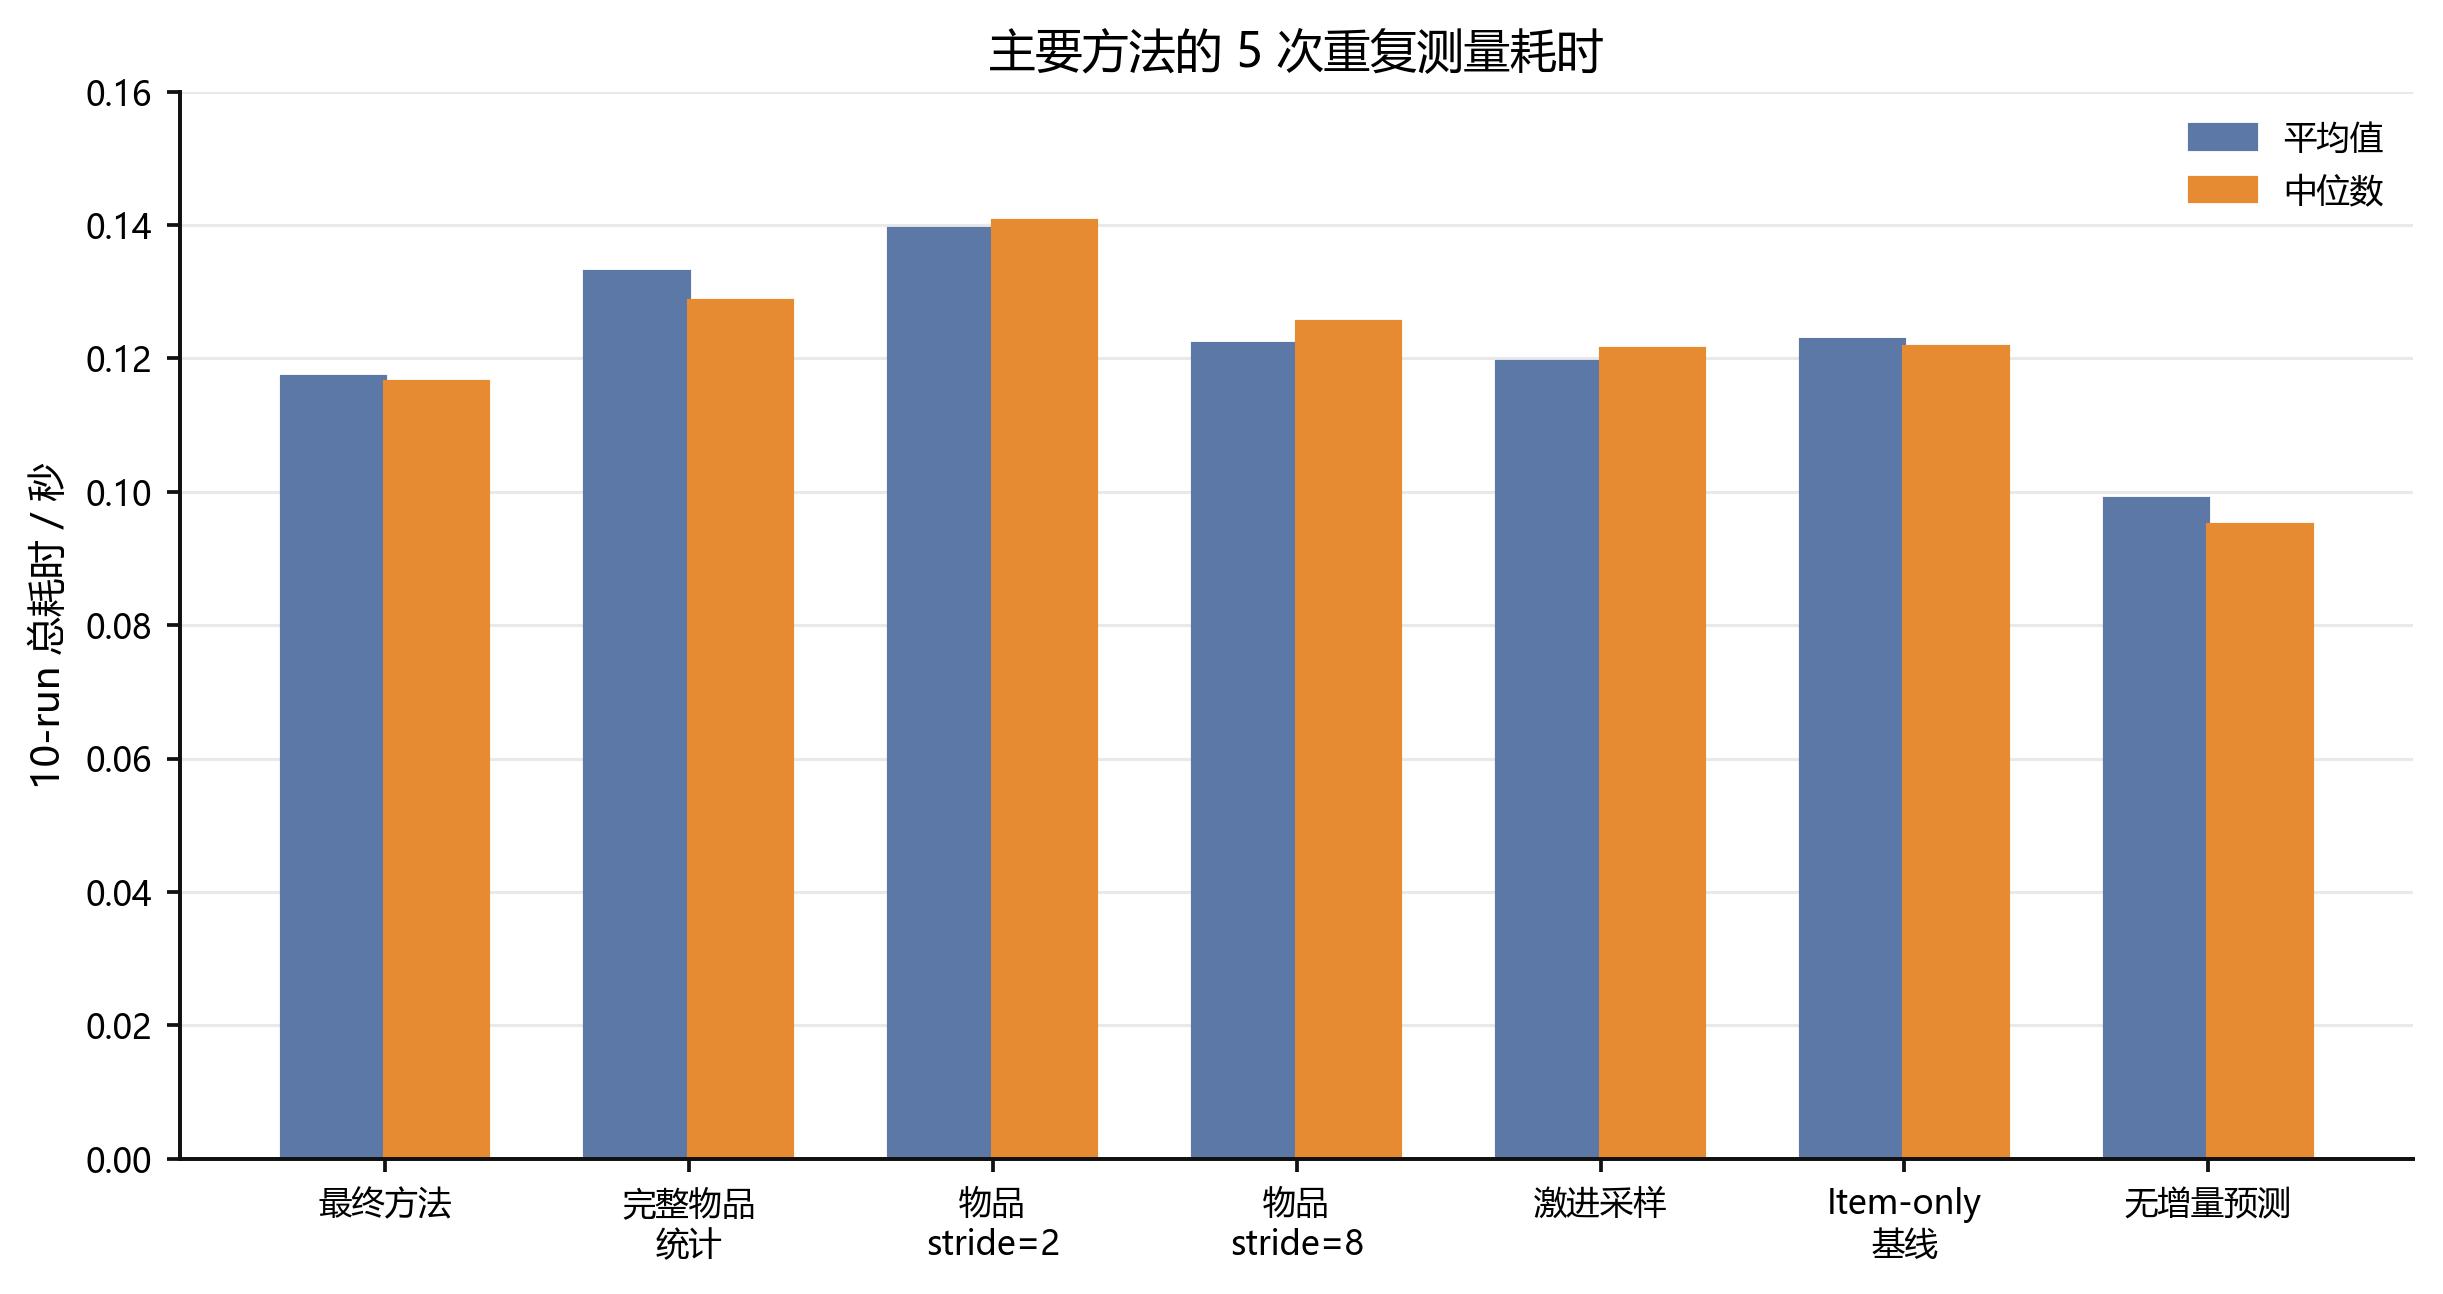
\includegraphics[width=0.90\linewidth]{main_method_runtime.png}
  \caption{主要方法的 5 次重复测量耗时。图中不绘制误差横线，柱高仅表示平均值和中位数。}
  \label{fig:runtime}
\end{figure}

\Cref{tab:main} 和 \Cref{fig:runtime} 显示，最终方法并不是 RMSE 最低的方案，但它在速度和精度之间取得了更好的折中。完整物品统计的 RMSE 最低，为 0.914846，但平均耗时比最终方法高约 13.5\%。stride=2 的 RMSE 也更低，为 0.916353，但平均耗时更高。激进采样和 item-only 基线的耗时接近最终方法，但 RMSE 明显更差。无增量预测最快，但没有任何 RMSE 改善，不能作为有效方案。

\begin{figure}[H]
  \centering
  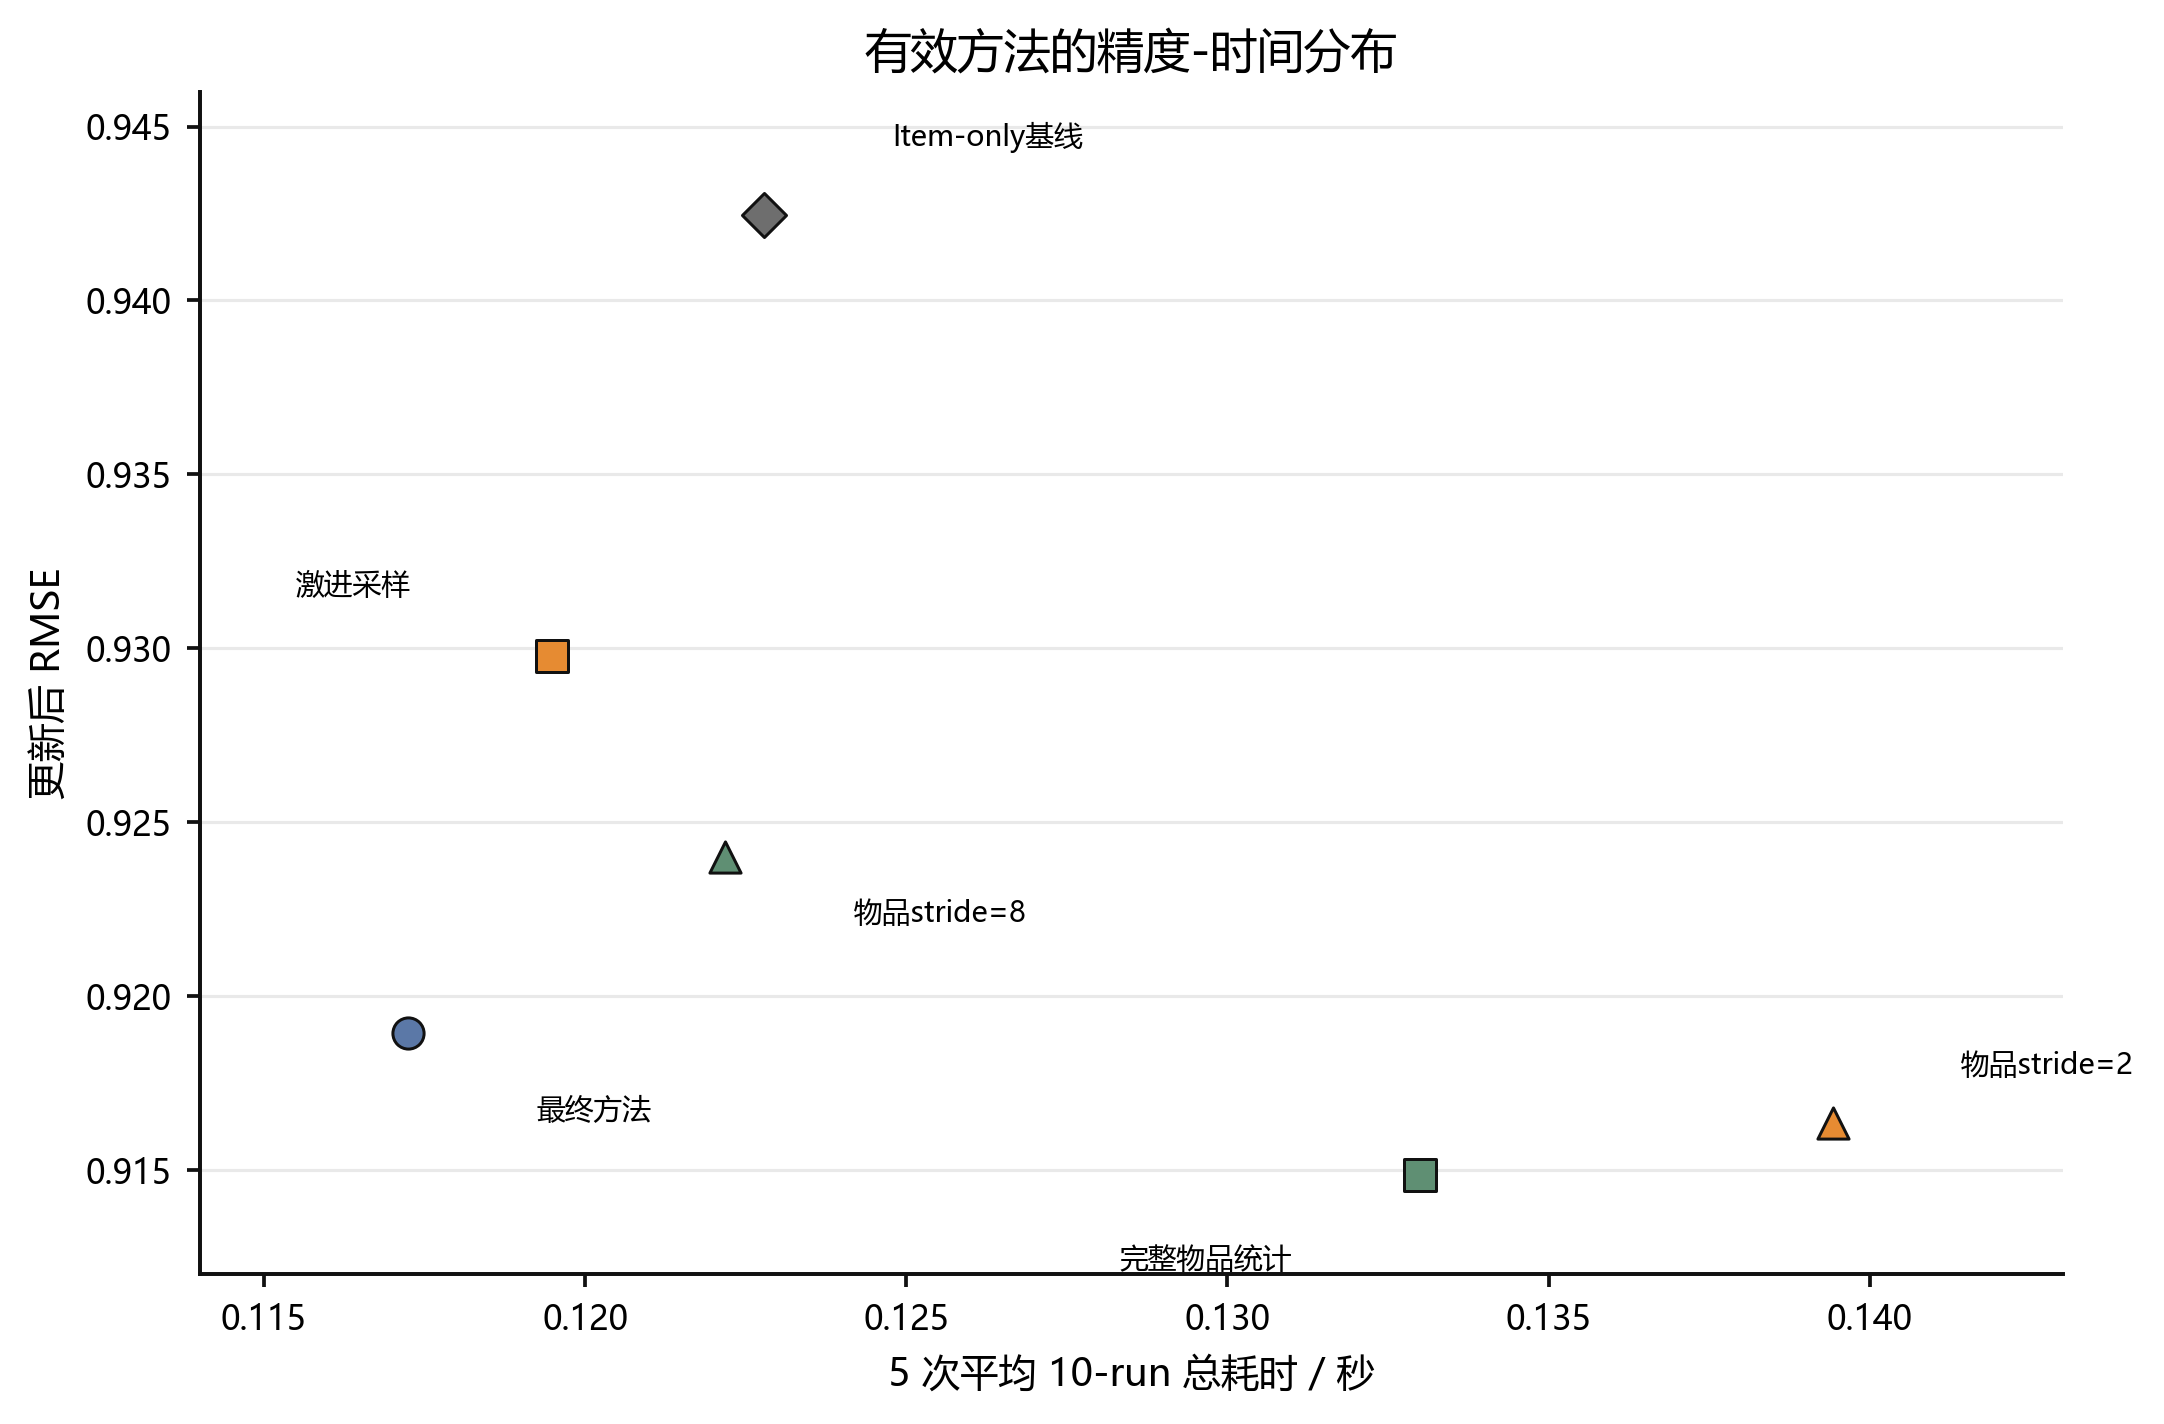
\includegraphics[width=0.86\linewidth]{tradeoff_scatter.png}
  \caption{有效方法的精度-时间分布。横轴越小表示越快，纵轴越小表示 RMSE 越低。}
  \label{fig:tradeoff}
\end{figure}

\Cref{fig:tradeoff} 进一步说明：若只追求 RMSE，完整物品统计和 stride=2 更靠下；若只追求速度，激进采样和 item-only 接近左侧，但精度损失更明显。最终方法处于较靠左且 RMSE 明显低于基线的位置，是本实验选择的提交点。

\section{采样强度扫描}

物品侧残差对 RMSE 贡献很大，但物品侧统计写入也占据更新成本。因此需要单独扫描采样强度。\Cref{tab:sampling} 和 \Cref{fig:sampling} 给出完整统计、stride=2、stride=4、stride=8、stride=16 的对比。这里 stride=4 即最终方法。

\begin{table}[H]
  \centering
  \caption{物品侧采样强度扫描。完整表示不跳过物品侧统计样本。}
  \label{tab:sampling}
  \begin{tabular}{lrrrr}
    \toprule
    采样间隔 & 更新后 RMSE & 平均耗时 & 相对最终方法 RMSE & 相对最终方法耗时\\
    \midrule
    完整 & 0.914846 & 0.1330 & -0.004101 & +13.5\%\\
    2 & 0.916353 & 0.1394 & -0.002594 & +18.9\%\\
    4 & 0.918947 & 0.1172 & 0.000000 & 0.0\%\\
    8 & 0.924010 & 0.1222 & +0.005063 & +4.3\%\\
    16 & 0.929777 & 0.1195 & +0.010830 & +2.0\%\\
    \bottomrule
  \end{tabular}
\end{table}

\begin{figure}[H]
  \centering
  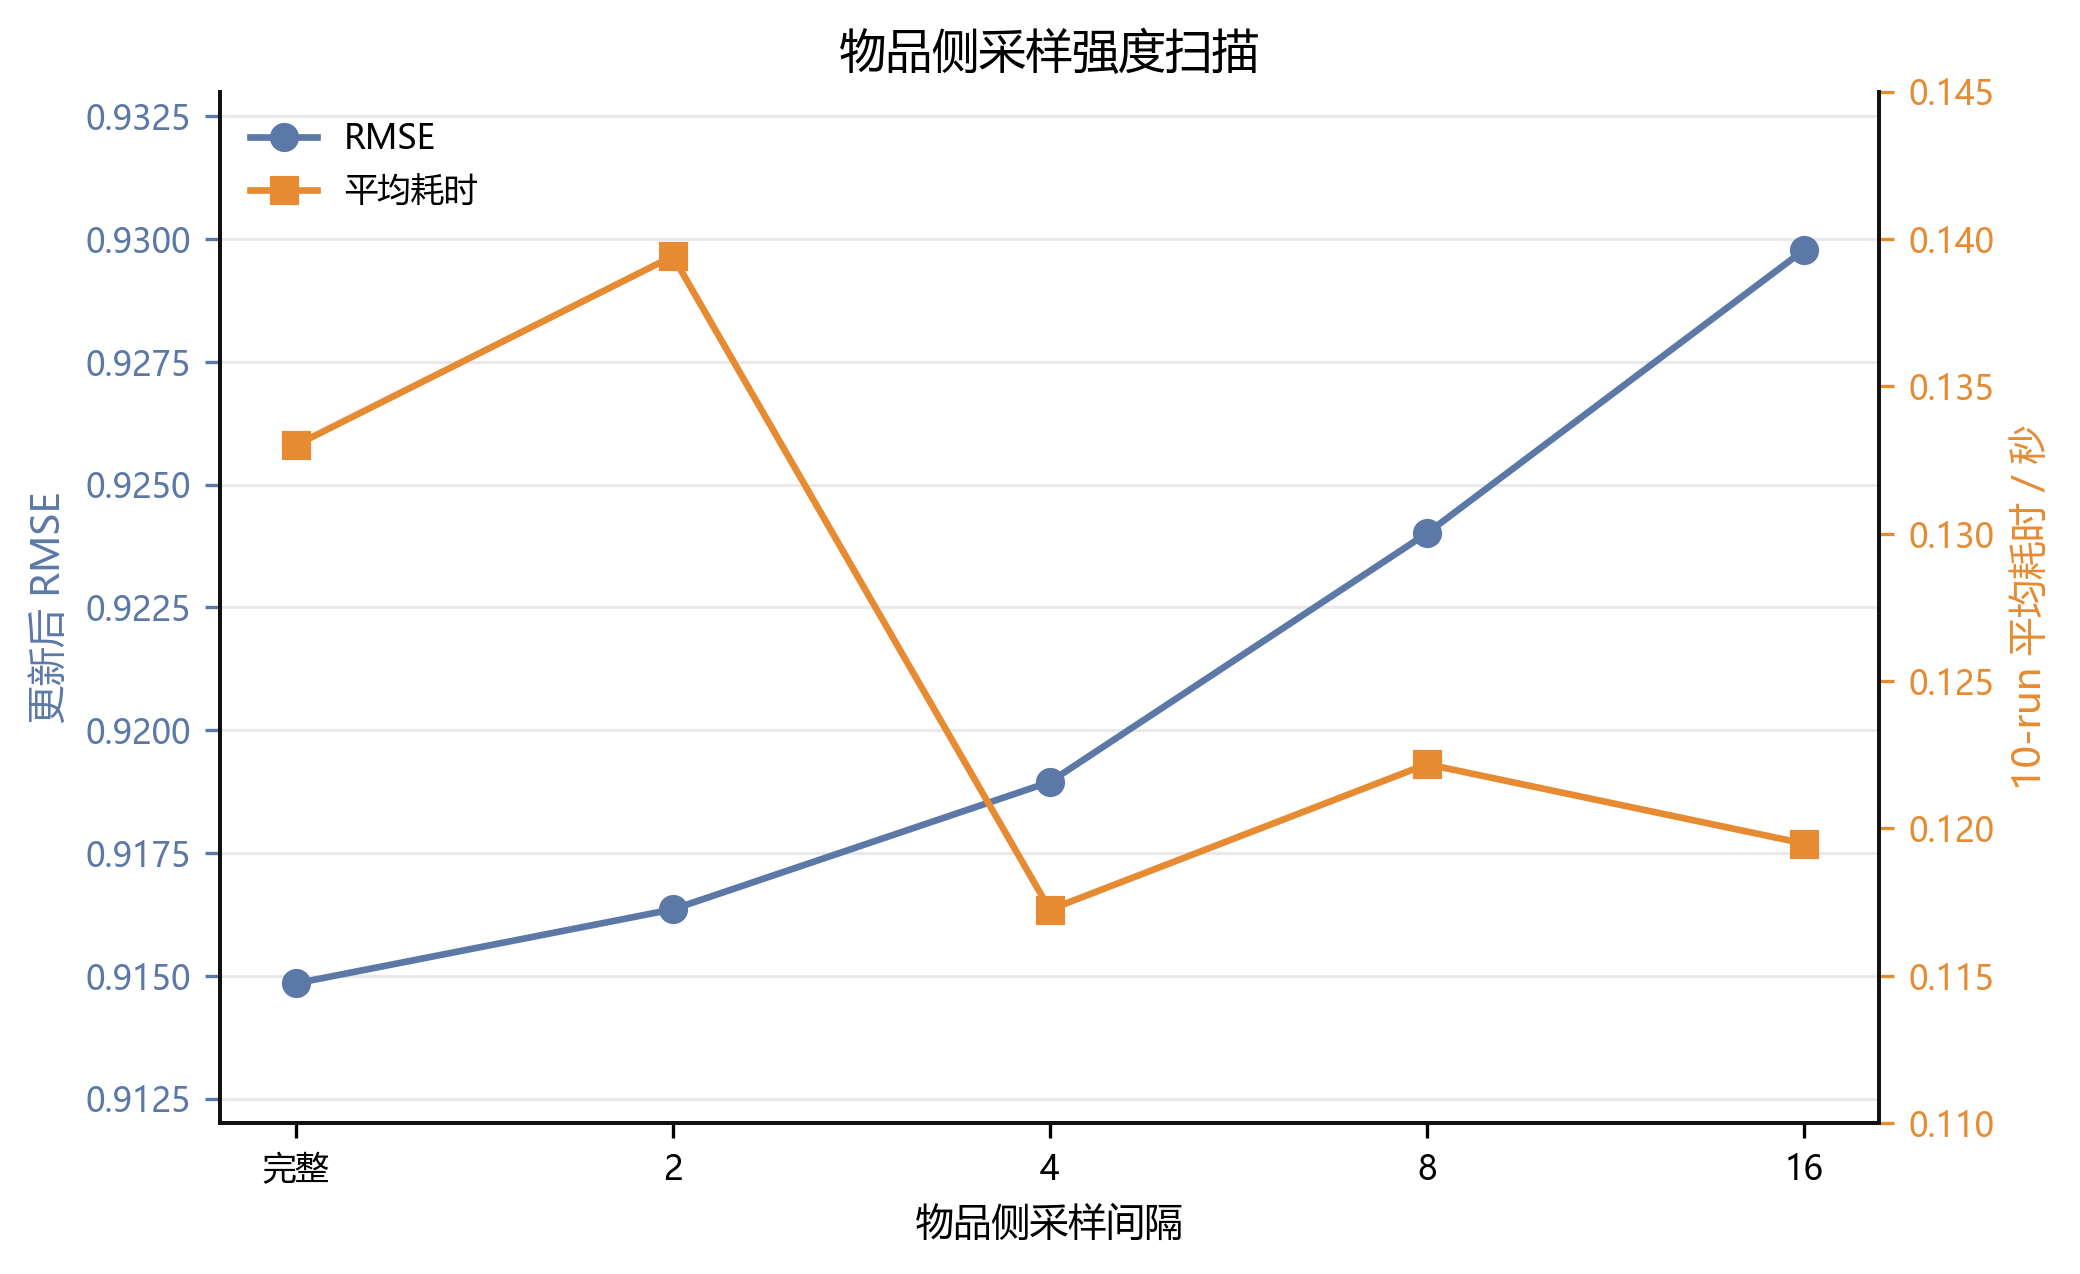
\includegraphics[width=0.82\linewidth]{sampling_sweep.png}
  \caption{物品侧采样间隔对 RMSE 和时间的影响。采样过密精度略好但更慢；采样过疏会使 RMSE 明显上升。}
  \label{fig:sampling}
\end{figure}

采样扫描的结论是：完整统计和 stride=2 对 RMSE 有收益，但时间代价较高；stride=8 和 stride=16 的时间收益并不稳定，且 RMSE 退化明显。最终选择 stride=4，是因为它保留了大部分物品残差信号，同时显著缩短统计写入路径。

\section{组件消融}

为了确认最终模型不是偶然调参结果，本实验对主要组件做了消融。每个消融只改变一个模型成分或一个成分组合，其余流程保持不变。\Cref{tab:ablation} 给出结果，\Cref{fig:ablation} 展示相对最终方法的 RMSE 损失。

\begin{table}[H]
  \centering
  \caption{关键组件消融。RMSE 增量越大，说明被移除组件越重要。}
  \label{tab:ablation}
  \begin{tabular}{lrrrr}
    \toprule
    消融设置 & 更新后 RMSE & RMSE 增量 & 平均耗时 & 中位数\\
    \midrule
    去物品残差 & 0.989332 & +0.070385 & 0.1127 & 0.1192\\
    去先验和计数 & 0.967422 & +0.048475 & 0.1152 & 0.1126\\
    去计数特征 & 0.950416 & +0.031469 & 0.1276 & 0.1198\\
    去用户分段先验 & 0.936505 & +0.017558 & 0.1187 & 0.1221\\
    去用户残差 & 0.928430 & +0.009483 & 0.1291 & 0.1256\\
    \bottomrule
  \end{tabular}
\end{table}

\begin{figure}[H]
  \centering
  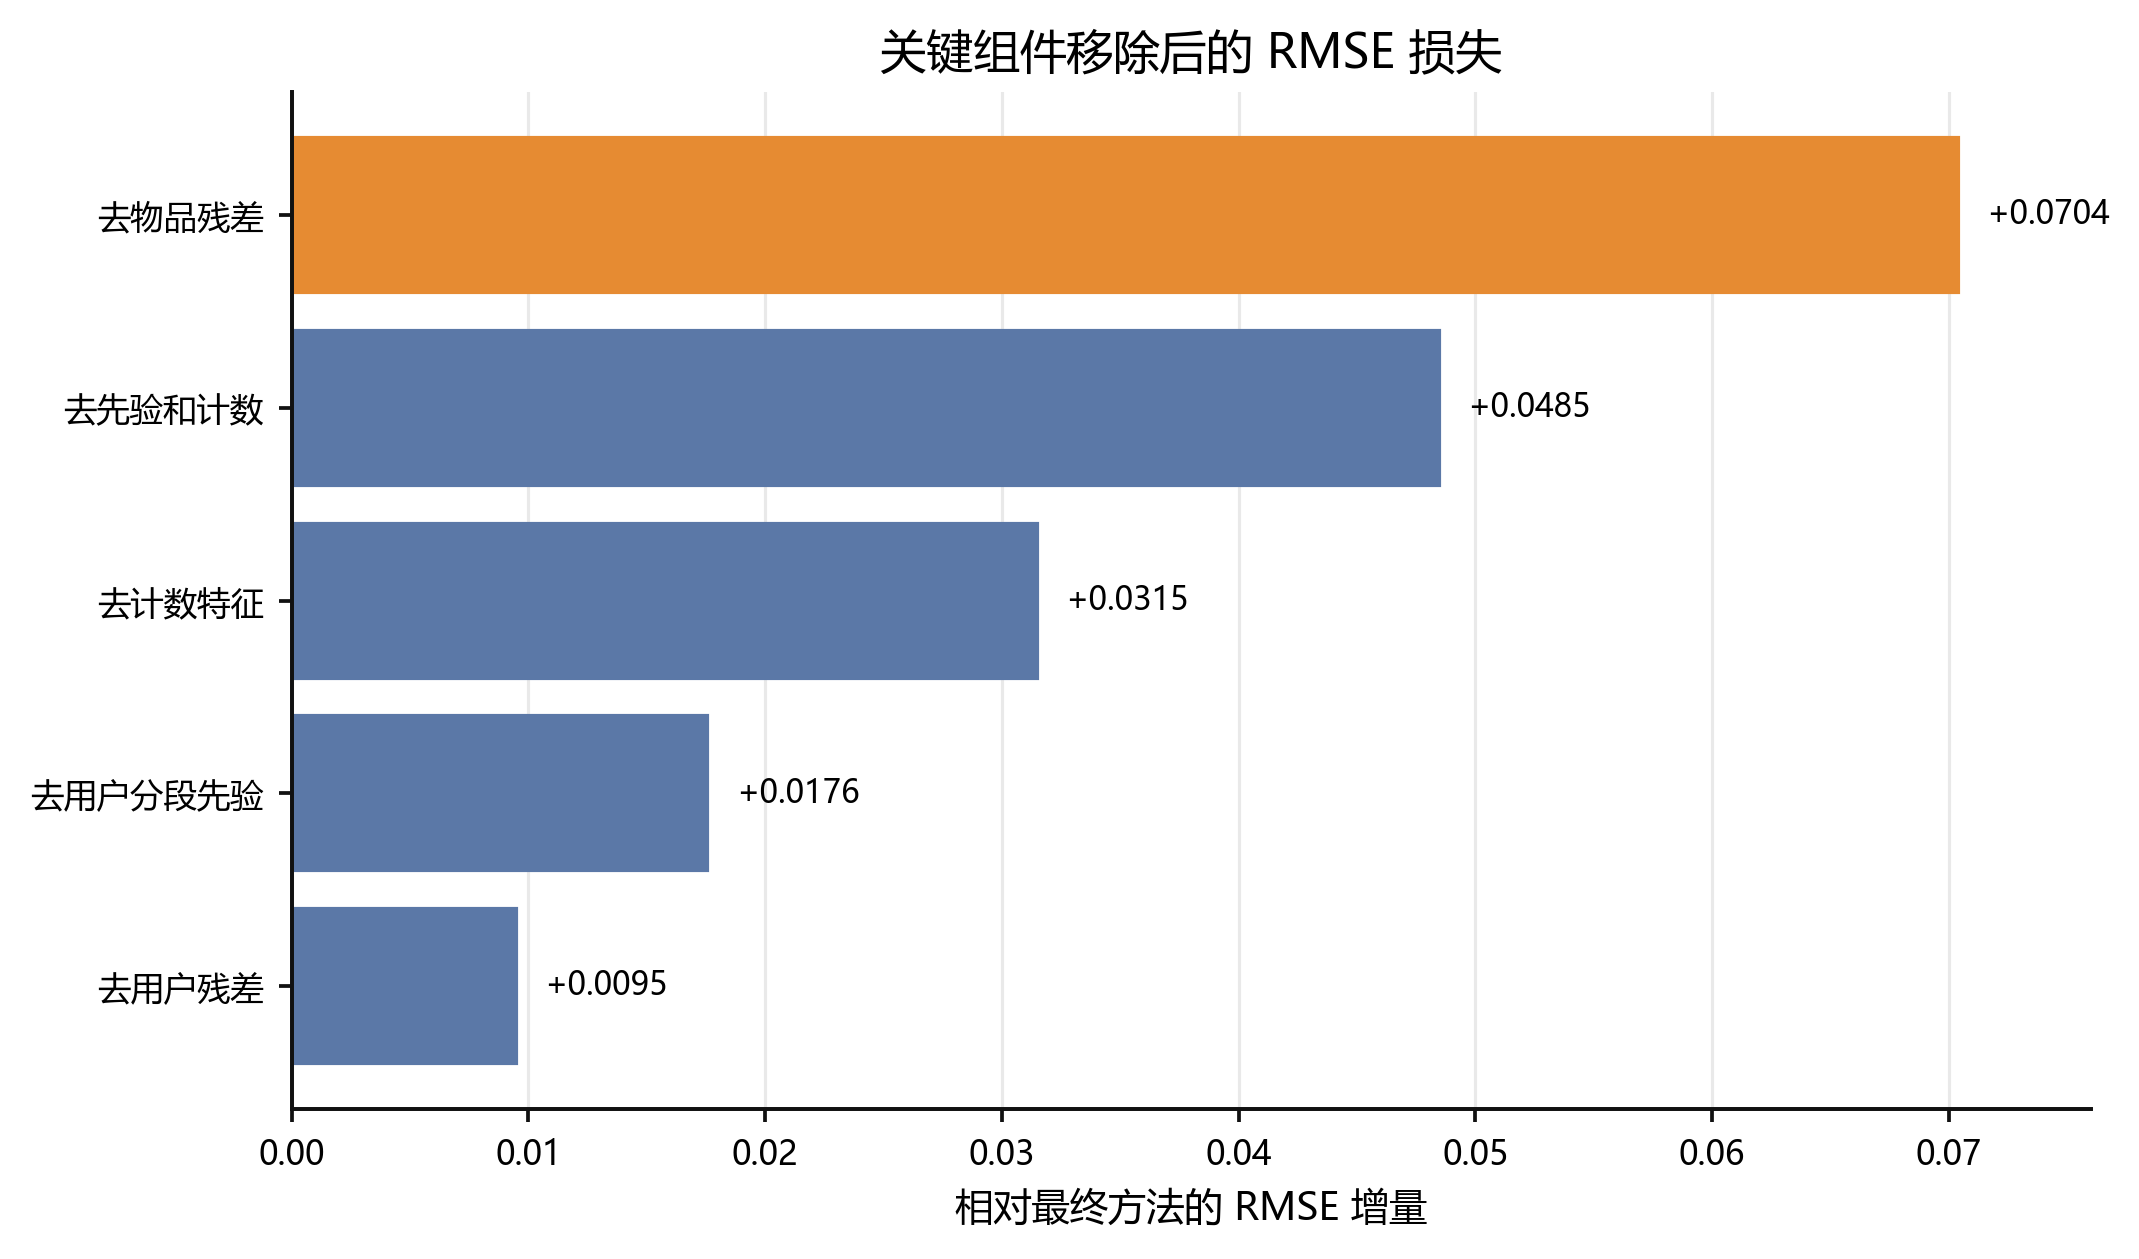
\includegraphics[width=0.82\linewidth]{ablation_rmse_delta.png}
  \caption{移除关键组件后的 RMSE 损失。物品残差是最重要的单项信号，计数特征和用户分段先验用于提升长尾稳定性。}
  \label{fig:ablation}
\end{figure}

消融结果有三点含义。第一，物品残差是主要精度来源，移除后 RMSE 上升 0.070385，几乎回到较弱基线。第二，计数特征和 shrinkage 不是微小超参，它们决定低频项如何回归到稳定估计；移除计数特征会使 RMSE 上升 0.031469。第三，用户残差的边际收益小于物品残差，但仍有可观贡献，说明用户侧信号较稀疏，需要依赖分段先验和 shrinkage 才能稳定发挥作用。

\section{时间稳定性}

当前评测环境存在短时调度波动，因此本文使用 5 次重复测量的均值和中位数，而不是单次最好值。\Cref{fig:repeat} 展示主要方法的 5 次时间序列。最终方法的五次结果集中在 0.1137--0.1247 s，波动小于完整物品统计和 item-only 基线。完整物品统计第一轮较慢，说明更重的刷新和写入路径对环境状态更敏感。

\begin{figure}[H]
  \centering
  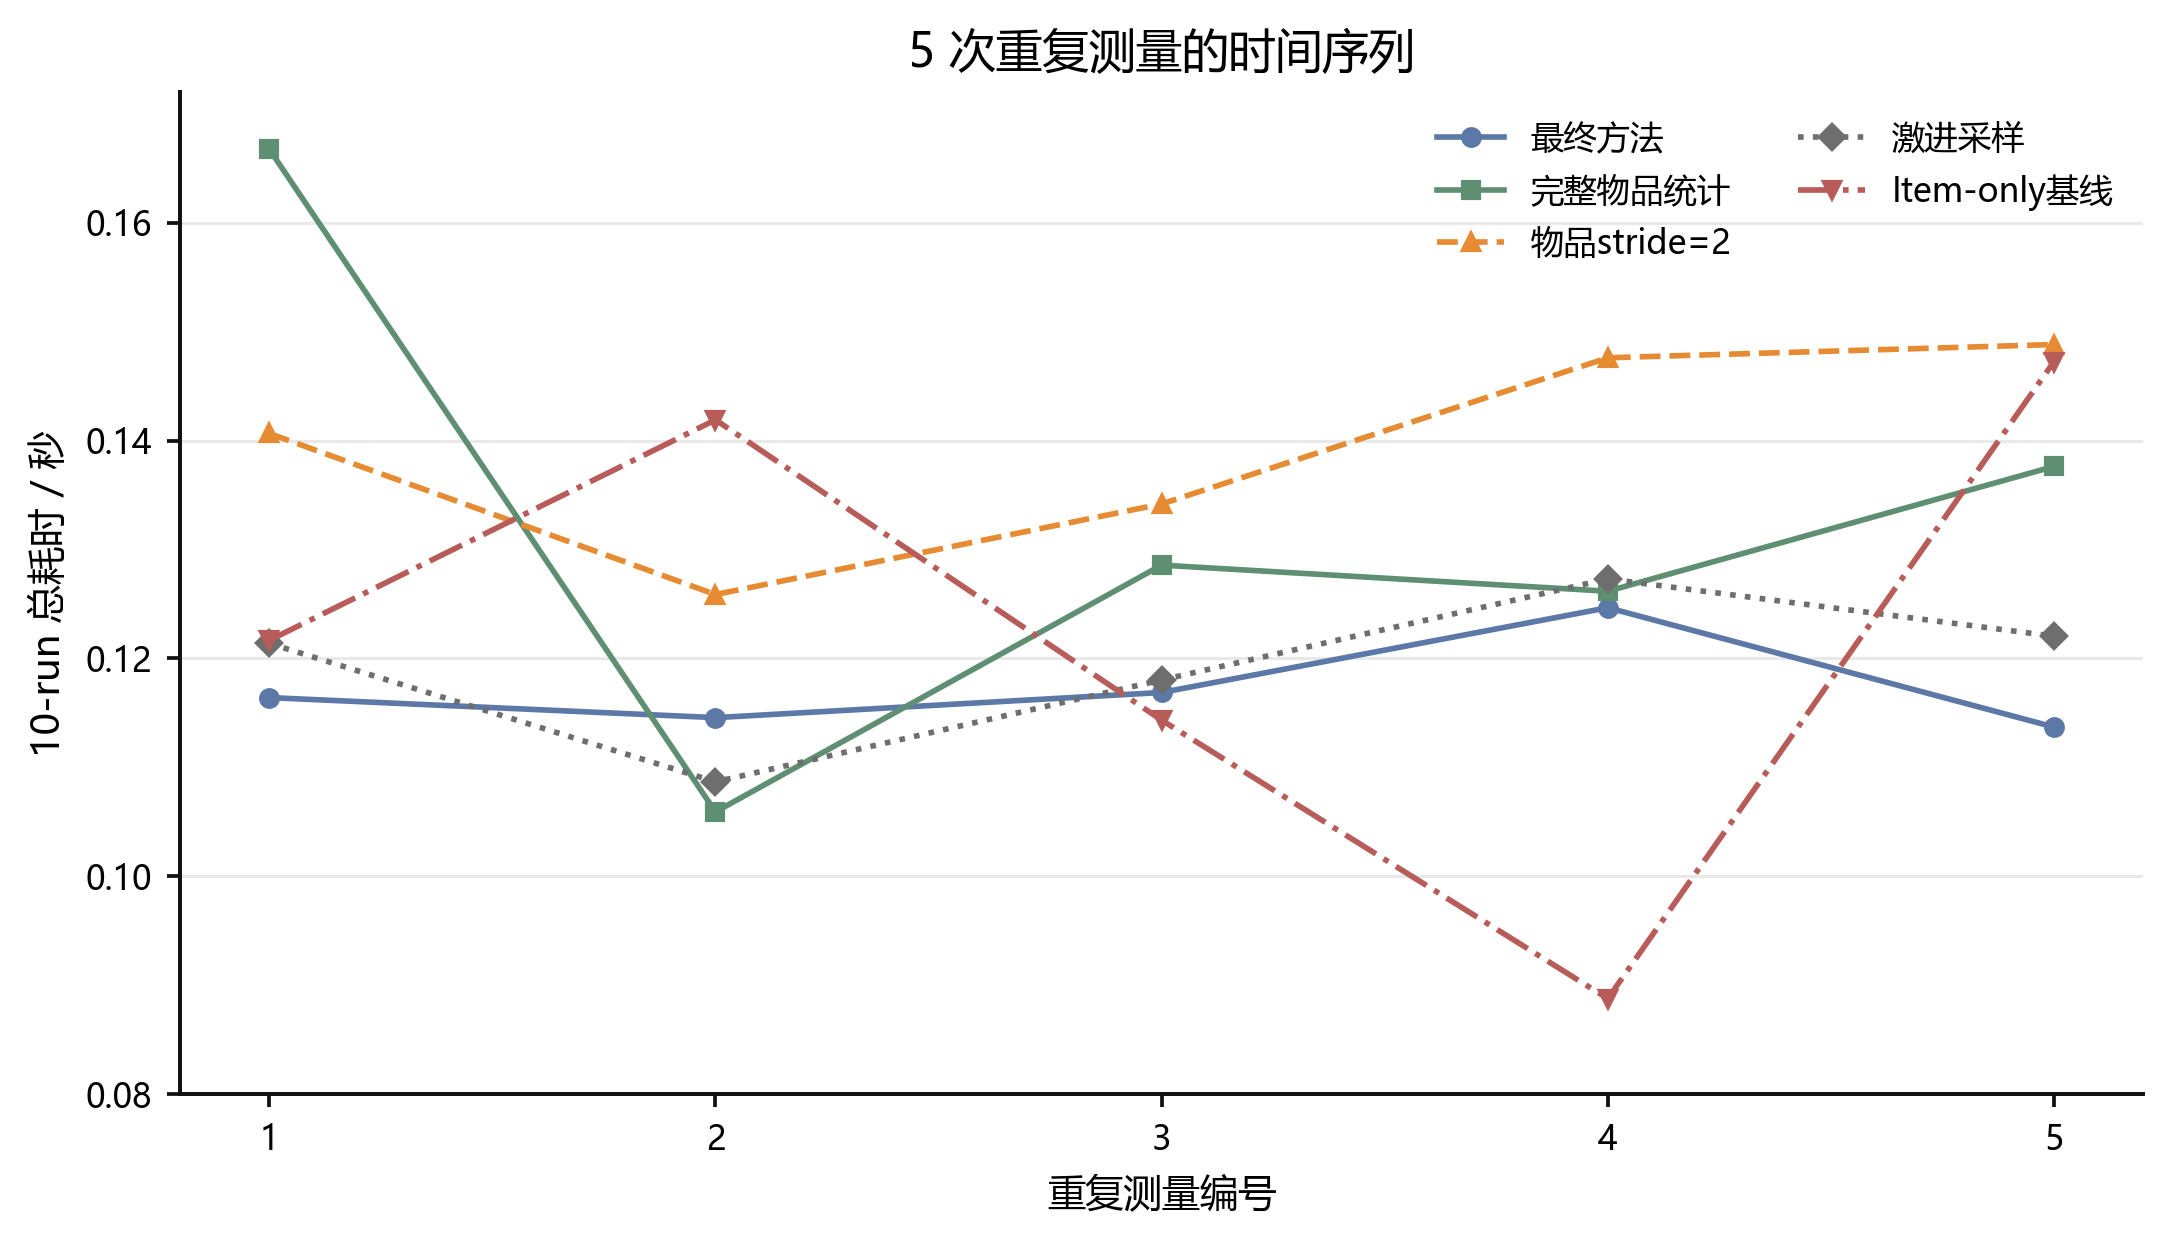
\includegraphics[width=0.86\linewidth]{repeat_sequence.png}
  \caption{主要方法的 5 次重复测量时间序列。每个点是一轮 10-run 总耗时。}
  \label{fig:repeat}
\end{figure}

\section{复杂度分析}

\Cref{tab:complexity} 先从渐进复杂度和主导常数比较直接 SVD 更新与最终方法，随后 \Cref{fig:complexity} 将关键热路径的操作量压缩可视化。二者共同说明：本方案的速度收益主要来自移除预测阶段的高维点积，并减少更新阶段的随机统计写入。

\begin{table}[H]
  \centering
  \caption{最终方法与直接 SVD 更新的复杂度比较。$N$ 为增量样本数，$M$ 为测试样本数，$I$ 为物品数，$d=1024$ 为隐向量维度。}
  \label{tab:complexity}
  \begin{tabular}{lll}
    \toprule
    阶段 & 直接 SVD 更新 & 最终方法\\
    \midrule
    增量误差计算 & $O(Nd)$ & $O(N)$，并通过采样降低常数\\
    参数更新 & $O(Nd)$ 写隐向量 & 写残差和与计数\\
    分数刷新 & 无缓存或重算点积 & $O(I+\#U_{\mathrm{touched}})$\\
    测试预测 & $O(Md)$ & $O(M)$\\
    主要瓶颈 & 大向量随机访存 & 小数组访问与顺序刷新\\
    \bottomrule
  \end{tabular}
\end{table}

\begin{figure}[H]
  \centering
  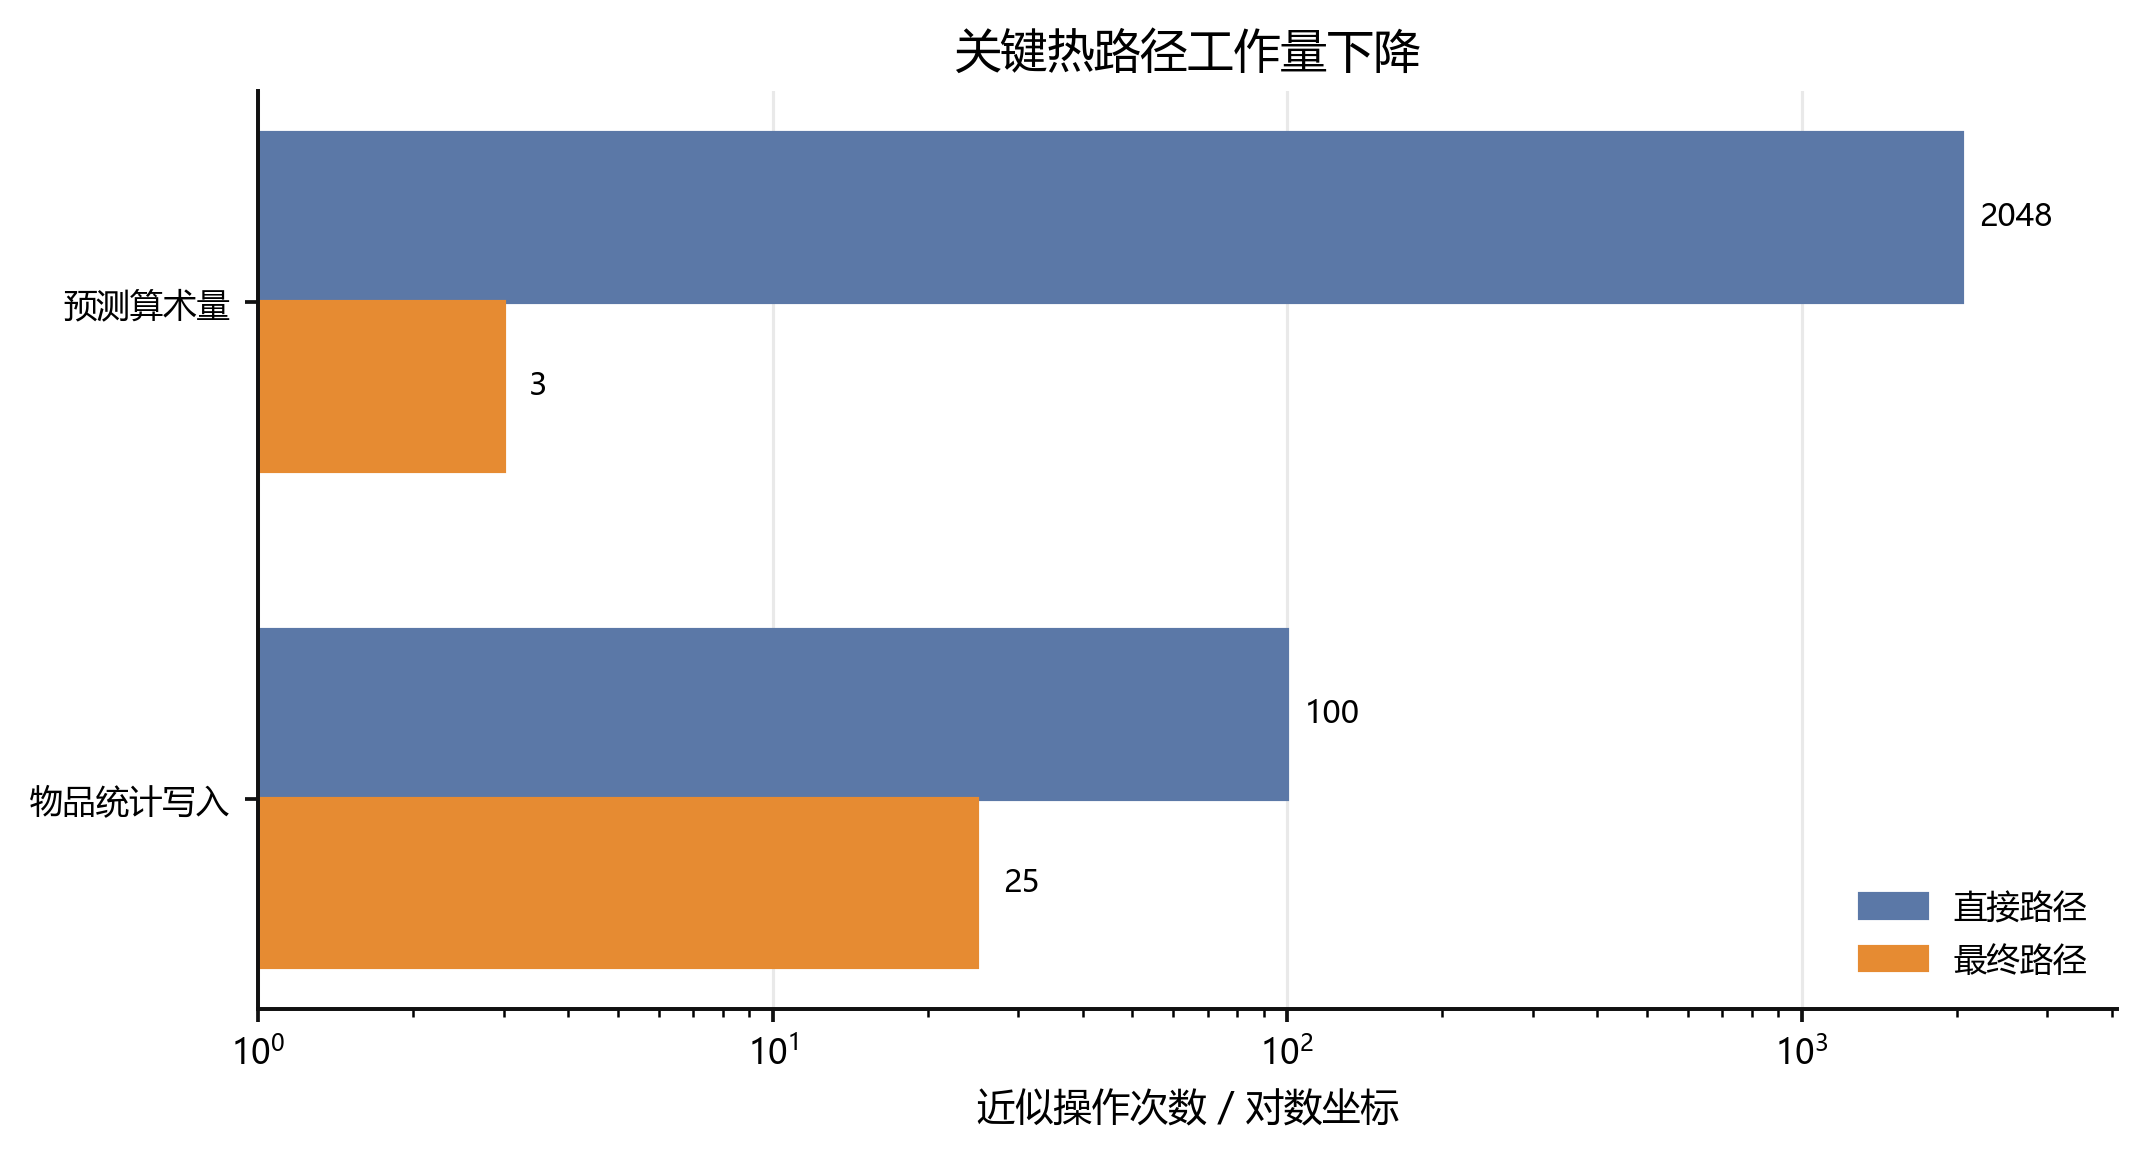
\includegraphics[width=0.82\linewidth]{complexity_reduction.png}
  \caption{关键热路径工作量下降。横轴采用对数坐标，因此最终预测路径的 3 次近似操作可以清楚显示。}
  \label{fig:complexity}
\end{figure}

\Cref{fig:complexity} 用对数坐标展示两条热路径的变化。预测阶段从完整点积的约 2048 次乘加相关操作压缩为 3 次左右的数组读取和加法；物品侧统计写入则由每 100 条样本写 100 次降到约 25 次。该复杂度变化解释了为什么最终方法能在 RMSE 显著改善的同时保持较低耗时。

\section{风险与取舍}

最终方法的主要风险是放弃了高维交互项，无法表达某个用户对某类物品的细粒度偏好变化。因此，它的 RMSE 不如完整物品统计或更密采样方案低。选择最终方法的原因是评测目标同时包含速度和有效性：完整统计虽然更准，但时间更高；更激进采样虽然时间接近，但 RMSE 接近失效边界；item-only 基线速度不稳定且精度明显不足。

另一个风险是过度依赖本地评测结构。开发中曾验证过跨轮状态复用会让重复评测更快，但它依赖同一进程重复运行相同数据，不属于稳健的增量算法。最终方案明确放弃该技巧，每轮按接口正常加载、更新和预测。这样牺牲了部分本地极限速度，但降低了隐藏评测中因批次变化而复用错误状态的风险。

\section{结论}

本实验最终采用采样残差校准，而不是完整 SVD 增量 SGD。扩展后的 12 组方法和消融实验表明：物品残差是最强信号，计数特征和用户分段先验提供稳定化收益，采样间隔需要在统计方差和随机写入之间折中。最终方法在当前环境下将 RMSE 从 1.023239 降至 0.918947，5 次重复测量的 10-run 平均耗时为 0.1172 s。后续若进一步追求 RMSE，可考虑在不显著增加预测开销的前提下加入极少量交互特征；若进一步追求速度，应优先优化统计刷新和内存布局，而不是恢复 1024 维点积。

\begin{thebibliography}{9}

\bibitem{task2spec}
课程组. \emph{实验一：增量 SVD 矩阵分解性能优化 / Track1 要求文档}. 2026.

\bibitem{harper2015movielens}
F. Maxwell Harper and Joseph A. Konstan.
\newblock The MovieLens Datasets: History and Context.
\newblock \emph{ACM Transactions on Interactive Intelligent Systems}, 5(4), 2015.

\bibitem{koren2009matrix}
Yehuda Koren, Robert Bell, and Chris Volinsky.
\newblock Matrix Factorization Techniques for Recommender Systems.
\newblock \emph{IEEE Computer}, 42(8):30--37, 2009.

\bibitem{koren2009bellkor}
Yehuda Koren.
\newblock The BellKor Solution to the Netflix Grand Prize.
\newblock \emph{Netflix Prize Documentation}, 2009.

\end{thebibliography}

\end{document}
